\documentclass[10pt]{article}
\usepackage[a4paper,margin=2cm]{geometry}
\usepackage{amsmath,amssymb,booktabs,graphicx,enumitem}
\usepackage[T1]{fontenc}\usepackage{lmodern}
\usepackage[font=small]{caption}\usepackage{placeins}
\setlength{\parindent}{0pt}\setlength{\parskip}{5pt}
\newcommand{\bs}{\beta^\star}\newcommand{\E}{\mathbb E}
\title{Unlearning and untraining with squared loss in a diagonal network:\\ setup, theory and results so far}
\author{}\date{25 November 2026}
\begin{document}\maketitle

\section{Setup}
\textbf{Network.} $f(x)=x^\top\beta$ with $\beta=u^2-v^2$ (entrywise), $u,v\in\mathbb R^d$, started at $u=v=k^{1/4}/2$ with $k=10^{-5}$, so $\beta=0$.

\textbf{Data.} The $d$ coordinates split into retain, shared and forget blocks of sizes $(d_r,d_{sh},d_f)$. A retain-class input is $\mathcal N(0,1/d)$ on the retain and shared blocks and zero elsewhere; a forget-class input likewise on the shared and forget blocks. The teacher $\bs$ has entries $\pm\rho^{-1/2}$ with probability $\rho=0.2$, else $0$. Labels are $y=x^\top\bs+\varepsilon$, $\varepsilon\sim\mathcal N(0,\sigma^2)$.

\textbf{Samples.} $R_{\rm full}$: retain-class samples. $F_{\rm full}$: forget-class samples. $F\subset F_{\rm full}$: the samples to forget. $R\subset R_{\rm full}$: retain samples used in finetuning. Each class has $\alpha$ samples per coordinate it sees.

\textbf{Pipeline.} \emph{Pretraining}: gradient descent on $\frac12\sum_{R_{\rm full}\cup F_{\rm full}}(x_i^\top\beta-y_i)^2$ until convergence. \emph{Rescaling}: $u,v\to\sqrt S\,u,\sqrt S\,v$. \emph{Finetuning}: gradient descent on
\[
\tfrac{\mu_r}2\sum_{i\in R}(x_i^\top\beta-y_i)^2+\text{(forget term on $F$)} .
\]
Time is $t=\text{step size}\times\text{steps}$; the step size is $0.01$.

\textbf{Forget terms.} Retain only (none). Forget-to-zero: $\frac{\mu_f}2\sum_F(x_i^\top\beta)^2$. Forget-to-noise: targets $\xi_i\sim\mathcal N(0,1)$. Negated target: targets $b\,y_i$, $b=-0.5,-1$. Signed: $-\frac{\mu_f}2\sum_F(x_i^\top\beta-y_i)^2$ with the retain term. Pure ascent: the same without it.

\textbf{References.} \emph{Ideal untraining}: the pretraining recipe on $R_{\rm full}\cup(F_{\rm full}\setminus F)$. \emph{Ideal unlearning}: the pretraining recipe on $R_{\rm full}$.

\textbf{Metrics} (mean squared error). (1) fresh retain-class inputs, against $x^\top\bs$; (2) the samples $F$, against their labels; (3) the left-over samples $F_{\rm full}\setminus F$, against their labels; (4) fresh forget-class inputs, against $x^\top\bs$. Also the distance $\|\beta-\beta_{\rm ref}\|^2/d$ to each reference.

\textbf{Baseline.} Blocks $\propto(1,0.4,1)$, $\alpha=0.3$, $|F|=\frac12|F_{\rm full}|$, $R=R_{\rm full}$, $\sigma=0$, $S=1$, $\mu_r=\mu_f=1$ (signed: $\mu_f=0.5$), full batch, no weight decay, $d=3000$, 5 seeds.

\section{Implicit bias}
\textbf{Mirror flow.} For any loss $L$ of the predictions $X^\top\beta$, gradient flow on $(u,v)$ gives $\dot u=-2u\,\nabla_\beta L$, $\dot v=+2v\,\nabla_\beta L$. Hence $uv$ is constant, and with $c=2uv$ (the same for all coordinates, $c=\sqrt k/2$),
\begin{equation}\label{mf}
\beta=c\,\sinh\theta,\qquad\dot\theta=-4\,\nabla_\beta L,\qquad\text{so }\theta(t)-\theta(0)\in\operatorname{span}X .
\end{equation}
\textbf{End point of a stage.} If a stage starts at $\beta_0$ with scale $c$ and ends fitting its targets $t$ on its samples $X$, then, with $\psi_c'(\beta)=\operatorname{arcsinh}(\beta/c)$ and $D_c$ the Bregman divergence of $\psi_c$,
\begin{equation}\label{proj}
\beta_{\rm end}=\arg\min_\beta D_c(\beta,\beta_0)\quad\text{s.t.}\quad X^\top\beta=t .
\end{equation}
(Its optimality conditions are \eqref{mf} and the constraints.) Small $c/|\beta|$ is the rich regime: for $\beta,\beta_0$ of the same sign and $\gg c$, $D_c\approx|\beta|\log\frac{|\beta|}{|\beta_0|}-|\beta|+|\beta_0|$, independent of $c$; a coordinate grown from zero costs $\approx|\beta|\log\frac{1}{c}$. Large $c/|\beta|$ is the lazy regime: $D_c\approx(\beta-\beta_0)^2/2c$.

\textbf{What changes $c$.}
\begin{center}\small\begin{tabular}{@{}lll@{}}\toprule
operation & effect & source\\\midrule
rescaling by $S$ & $\beta\to S\beta$, $c\to Sc$ & direct\\
weight decay $\frac\lambda2(\|u\|^2+\|v\|^2)$ for a time $T$ & $c\to c\,e^{-2\lambda T}$; kept on forever: penalty $\frac\lambda2|\beta|$ & direct\\
SGD with step $\gamma$, batch gradient $G$ & $c_j\to c_j\prod_{\rm steps}(1-4\gamma^2G_j^2)$ & Even et al.\ 2023\\\bottomrule
\end{tabular}\end{center}
\textbf{Local rule.} By \eqref{mf}, $\dot\beta_j=-4\sqrt{\beta_j^2+c^2}\,\nabla_jL=-4(u_j^2+v_j^2)\nabla_jL$. To first order, finetuning moves $\beta$ by $\Delta\beta_j=(u_j^2+v_j^2)\,(X\lambda)_j$: the squared weight norm of a coordinate at the pretrained model decides how much it moves. After small-$k$ pretraining this is $|\beta_j|$ on learned coordinates and $c$ elsewhere.

\textbf{Untied layers} (Azulay et al.\ 2021). For $w=u_+v_+-u_-v_-$ per coordinate, write $R=\frac12(u_+^2+v_+^2+u_-^2+v_-^2)$. Then $\dot w=-2R\,\nabla L$, and $c^2=R^2-w^2$ is conserved, so \eqref{mf}--\eqref{proj} hold with this $c$. From $w=0$ with $u_+=u_-$, $v_+=v_-$ this is their Theorem 4.1 ($\sqrt k=2c=2(u_+^2+v_+^2)$). The general-start formula is my own derivation (their Appendix B was not in the copy I read), checked numerically. Our network is the case $u_\pm=v_\pm$. Multiplying one layer by $a$ and the other by $1/a$ keeps $w$ and raises $c$ on trained coordinates ($c\approx|w|\,|a^2-a^{-2}|/2$); this operation does not exist for $\beta=u^2-v^2$ and was not run.

\section{Large-$d$ theory}
$d\to\infty$ at fixed sample ratios. Derivation by the cavity method (add one coordinate, add one sample, first-order perturbation); not a proof.

\textbf{Pretrained model and references} (each an interpolation from zero). For one sample let $z=x^\top\bs$, $\zeta$ the prediction the model would make had it not seen the sample, and $g$ the sample's accumulated loss gradient. For one coordinate let $\eta$ be its Gaussian field. With $V=\E\,\partial\beta/\partial\eta<0$:
\begin{equation}\label{st}
\zeta+Vg=y,\qquad \theta+A(\beta-\bs)=-\eta,\quad\beta=c\sinh\theta,\qquad A=-\sum_a\alpha_a/V_a ,
\end{equation}
where $(z,\zeta)$ is Gaussian with the covariance of $(\bs,\beta)$, $\eta$ is Gaussian with variance $\sum_a\alpha_a\E g^2$, and the sums run over the sample groups $a$ (each $\alpha_ad$ samples) that touch the coordinate's block; $V_a$ averages over the blocks group $a$ touches. With weight decay kept on: $g=(\zeta-y)/(1-V)$, $A=\sum_a\alpha_a/(1-V_a)$, $\beta=\operatorname{soft}(\bs-\eta/A,\ \lambda/2A)$.

\textbf{Finetuning trajectory.} For one sample and one coordinate, at step $n$ of size $\delta$:
\begin{equation}\label{dyn}
p_n=\zeta_n+\sum_{l<n}R_\beta(n,l)\,g_l,\qquad g_n=w_n(p_n-t_n),\qquad
G_n=\eta_n+\sum_{l\le n}R_g(n,l)\,\beta_l+\mu_n\bs ,
\end{equation}
and $u\leftarrow u(1-2\delta G_n-\delta\lambda)$, $v\leftarrow v(1+2\delta G_n-\delta\lambda)$. Here $p_n$ is the prediction, $w_n$ the sample's loss weight, $t_n$ its target; $R_\beta(n,l)=\E\,\partial\beta_n/\partial\eta_l$, $R_g(n,l)=\sum_a\alpha_a\E\,\partial g_n/\partial\zeta_l$, $\mu_n=\sum_a\alpha_a\E\,\partial g_n/\partial z$. The pretrained model enters as step $l=0$, with $g_0$, $\partial\beta_0/\partial\eta_0$ and $\partial g_0/\partial\zeta_0=-1/V$ from \eqref{st}.

\textbf{Solver.} \eqref{st} is solved with fixed stratified Gaussian draws. Two independent Gaussian matrices are then drawn conditionally on reproducing $\zeta$ and $\eta$ of \eqref{st}, and \eqref{dyn} is run forward on them with tangent propagation for $R_\beta,R_g,\mu$. Cost grows as (steps)$^3$, so theory curves stop at $t=6$ (step $0.05$); simulations run to $t=40$. The pretraining trajectory uses \eqref{dyn} from zero.

\section{Runs}
27 configurations $\times$ 4 block settings $\times$ 7 losses; 5 simulation seeds and 3 theory runs each.
\begin{center}\small\begin{tabular}{@{}lll@{}}\toprule
varied & values & status\\\midrule
blocks $(d_r,d_{sh},d_f)\propto$ & $(1,0.4,1)$; $(0,1,0)$; $(1,0,1)$; $(1,1,1)$ & all\\
$|F|/|F_{\rm full}|$ & $0.1,\ 0.5,\ 0.9,\ 1$ & done\\
label noise $\sigma^2$ in pretraining & $0,\ 0.1,\ 0.5$ & done\\
fresh forget samples in finetuning (noise $0,0.1,0.5$) & & done\\
rescaling $S$ & $0.1,\ 0.3,\ 1,\ 3$ & done\\
$(\mu_r,\mu_f)$ & $(1,0.25),\ (1,1),\ (1,4)$ & running\\
$R$ = a quarter of $R_{\rm full}$ & & running\\
SGD (batch fraction $0.1$) in either stage & & running\\
weight decay $0.1,\ 0.3$ in either or both stages & & running\\
$\alpha=0.8,\ 1.5$ (with reused and fresh forget samples) & & running\\\bottomrule
\end{tabular}\end{center}
Changes from the agreed table: decay values $0.1,0.3$ (convergence needs $t\approx12/\lambda$); middle $\alpha=0.8$ (recovery threshold $\approx0.55$); the $\alpha\ge0.8$ runs use $d=2000$ and $t\le20$.

\section{Results}
\subsection{Theory against simulation}
Forget-to-zero and the two negated targets, all finished configurations: 2868 comparisons (six quantities, four times), $94\%$ within 2 standard errors, median gap $3.0\%$, 90th percentile $9.7\%$ (Figure~\ref{base}). Worst configuration: $S=3$ ($92\%$, median $4.6\%$).

\emph{Forget-to-noise} is much noisier: the outcome follows the empirical variance of the $\approx260$ noise targets. With 12 runs per side theory and simulation agree, except a $\approx10\%$ excess of theory on the left-over samples at $t\ge4$; simulations at $d=6000$ are closer (Figure~\ref{noise}).

\emph{Signed loss and pure ascent}: the pretrained model fits $F$, so the gradient is zero and theory predicts no motion. In simulation they diverge at $t\approx2$--$4$ from the $2\times10^{-4}$ training error left by pretraining. \emph{Retain only} does nothing.

Seed-to-seed scatter is large at $k=10^{-5}$: about $5\%$ on the pretrained error at $d=3000$.

\begin{figure}[!ht]\centering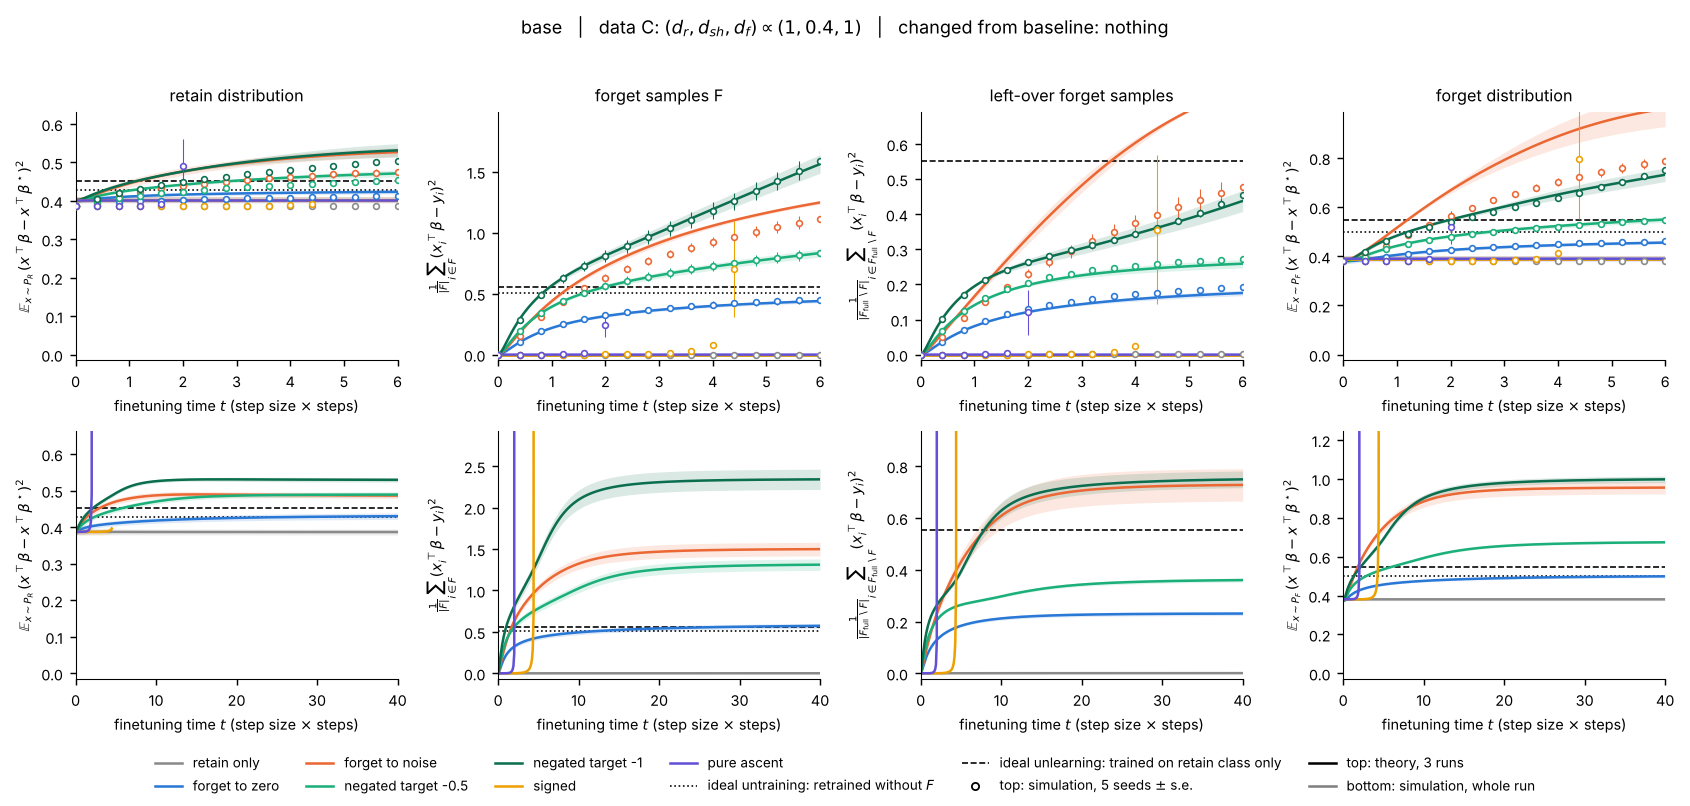
\includegraphics[width=\linewidth]{figs/base__C.png}
\caption{Baseline. Top: theory (lines) and simulation (markers) for $t\le6$. Bottom: simulation to $t=40$. The orange theory curve (forget-to-noise) is three unlucky runs; see Figure~\ref{noise}.}\label{base}\end{figure}
\begin{figure}[!ht]\centering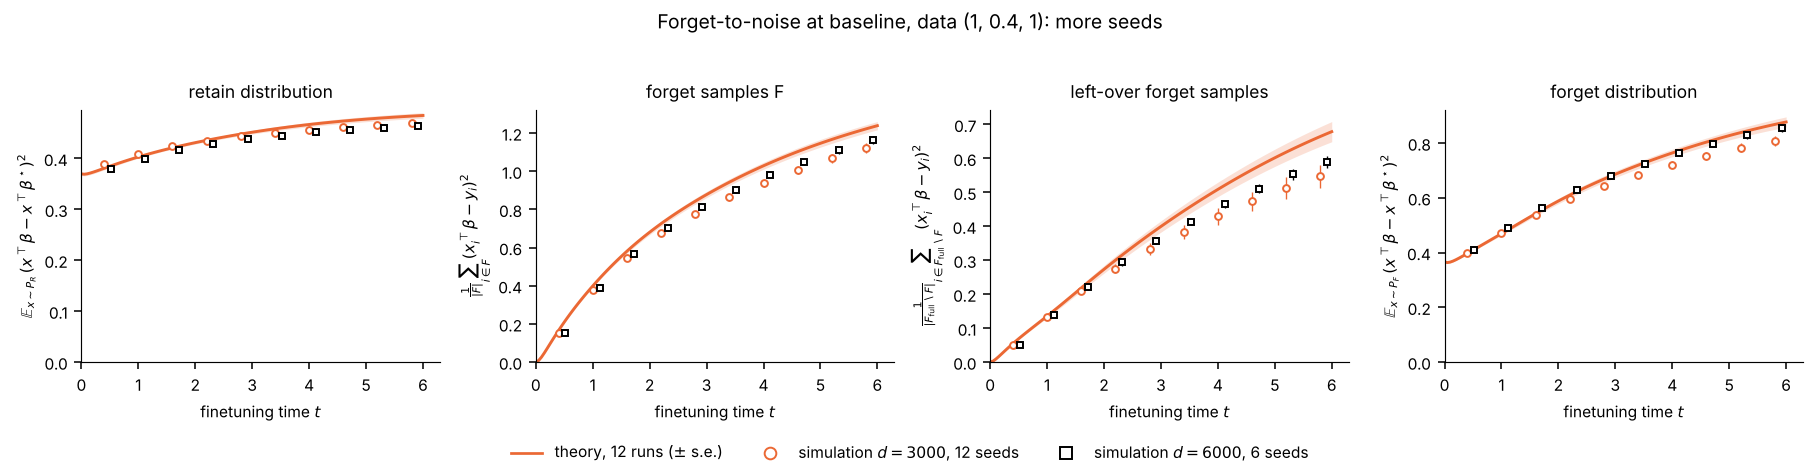
\includegraphics[width=\linewidth]{figs/noise_more_seeds.png}
\caption{Forget-to-noise at baseline with 12 runs per side.}\label{noise}\end{figure}

\subsection{Baseline, end of finetuning (simulation)}
\begin{center}\small\begin{tabular}{@{}lcccccc@{}}\toprule
& retain dist. & $F$ & $F_{\rm full}\setminus F$ & forget dist. & dist.\ to untraining & dist.\ to unlearning\\\midrule
pretrained & 0.387 & 0.000 & 0.000 & 0.381 & 0.207 & 0.290\\
ideal untraining & 0.429 & 0.507 & 0.000 & 0.499 & 0 & \\
ideal unlearning & 0.452 & 0.555 & 0.553 & 0.547 & & 0\\\midrule
forget-to-zero & 0.430 & 0.573 & 0.231 & 0.499 & 0.140 & 0.096\\
negated $-0.5$ & 0.489 & 1.311 & 0.360 & 0.674 & 0.260 & 0.249\\
negated $-1$ & 0.530 & 2.341 & 0.749 & 0.998 & 0.530 & 0.567\\
forget-to-noise & 0.486 & 1.499 & 0.727 & 0.955 & 0.657 & 0.736\\\bottomrule
\end{tabular}\end{center}
Smallest distance along the path (time reached): forget-to-zero $0.119$ ($t=2.3$) and $0.090$ ($t=11.7$); negated $-0.5$: $0.125$ ($0.8$) and $0.112$ ($2.2$); negated $-1$: $0.129$ ($0.4$) and $0.127$ ($0.9$). Negated targets pass near the same point 3--5 times sooner, then overshoot.

\subsection{Blocks, forget fraction, rescaling (forget-to-zero)}
\begin{center}\small\begin{tabular}{@{}lcccc@{}}\toprule
blocks $\propto$ & $(1,0,1)$ & $(1,0.4,1)$ & $(1,1,1)$ & $(0,1,0)$\\\midrule
retain error, pretrained $\to$ end & $0.374\to0.374$ & $0.387\to0.430$ & $0.356\to0.472$ & $0.068\to0.704$\\
distance to unlearning, start $\to$ end & $0.222\to0.012$ & $0.290\to0.096$ & $0.339\to0.187$ & $0.523\to0.395$\\
distance to untraining, start $\to$ best & $0.184\to0.094$ & $0.207\to0.119$ & $0.221\to0.135$ & $0.262\to0.196$\\\bottomrule
\end{tabular}\end{center}
With no shared block the retain error does not move (the forget gradient is zero on retain coordinates) and forget-to-zero converges to the retain-only model. With all coordinates shared, both classes together exceed the recovery threshold, the pretrained model is nearly the teacher, and every forget loss destroys the retain error.

\begin{figure}[!ht]\centering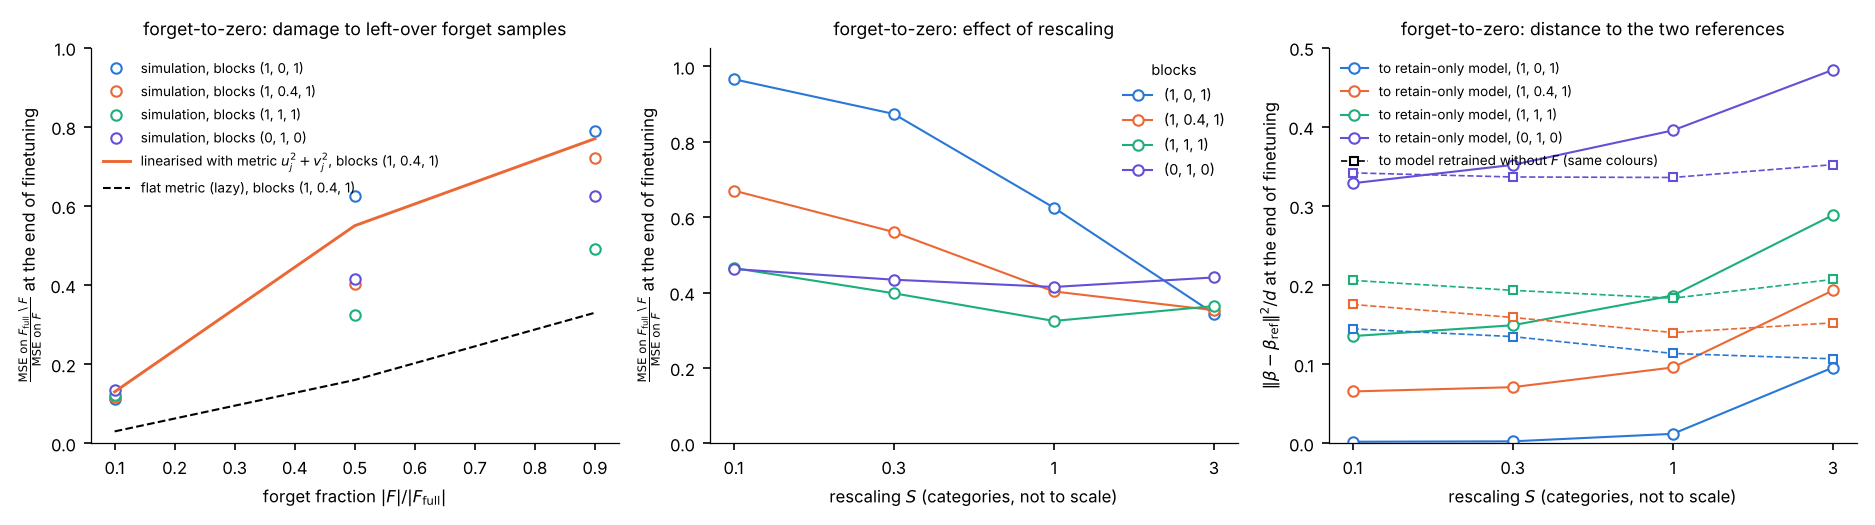
\includegraphics[width=\linewidth]{figs/summary.png}
\caption{Forget-to-zero at the end of finetuning. Left: error on the left-over samples relative to the error on $F$, against the forget fraction. Middle and right: against the rescaling $S$.}\label{sum}\end{figure}

\textbf{Forget fraction} (Figure~\ref{sum}, left). The ratio (error on $F_{\rm full}\setminus F$)/(error on $F$) is $0.12,\ 0.40,\ 0.72$ at $|F|/|F_{\rm full}|=0.1,0.5,0.9$. The local rule of Section 2 predicts $0.13,\ 0.55,\ 0.77$; a flat metric (lazy finetuning from the same model) gives $0.03,\ 0.16,\ 0.33$, equal to the forget samples per class coordinate. At $0.9$ and no shared block the distance to the retain-only model is $0.001$.

\textbf{Rescaling} (Figure~\ref{sum}, middle and right). Larger $S$ lowers the damage to left-over samples and raises the distance to the retain-only model; smaller $S$ does the opposite. Blocks $(1,0,1)$: ratio $0.97,\ 0.87,\ 0.63,\ 0.34$ and distance to the retain-only model $0.002,\ 0.002,\ 0.012,\ 0.096$ at $S=0.1,0.3,1,3$. So $S<1$ pushes towards unlearning and $S>1$ towards untraining. The distance to the retrained model changes little ($0.145\to0.107$).

\textbf{Label noise in pretraining.} All errors rise; the ratio above stays $0.40$ at $\sigma^2=0.1$; the ordering of losses is unchanged.

\textbf{Fresh forget samples.} Forget-to-zero on fresh samples raises the error on $F$ and on $F_{\rm full}\setminus F$ equally ($0.143$ and $0.137$): it cannot single out $F$. Distance to the retain-only model ends at $0.197$ (reused: $0.096$).

\section{Reading}
\begin{itemize}[nosep,leftmargin=1.2em]
\item Finetuning moves the coordinates the pretrained model uses (local rule). After small-$k$ pretraining these are few, so forgetting $F$ spreads to every input that shares them: unlearning. Spread over all coordinates (flat metric) it stays on the samples: untraining.
\item The spread is governed by (forget samples)/(effective number of coordinates that move); it grows with $|F|$ and falls with $S$.
\item The best forget target is the reference model's own prediction on $F$. Forget-to-zero wins here because the retain-only model predicts zero on forget inputs when no block is shared; with a shared block it is the wrong target and degrades accordingly.
\item No loss reaches the retrained model: best reduction of the distance $40$--$50\%$.
\end{itemize}

\section{Open}
\begin{itemize}[nosep,leftmargin=1.2em]
\item Why rescaling moves the spread as much as it does. I argued it should be weak (it leaves $c/|\beta|$ unchanged on every learned coordinate and only makes new coordinates cheaper by $\log S$); the data show a clear effect. Not resolved.
\item Predictions not yet tested (runs pending): weight decay and SGD shrink $c$ and should push towards unlearning; above the recovery threshold ($\alpha=0.8$) the retrained model equals the pretrained one, so untraining means doing nothing.
\item Residual theory--simulation gaps: $\approx10\%$ on left-over samples for forget-to-noise at $t\ge4$; negated $-1$ distances to the references about $14\%$ high in theory at $t=6$ in one check.
\item No theory for finetuning after SGD pretraining; for SGD finetuning only to $t=1.2$.
\item No end-point ($t\to\infty$) theory curves for finetuning yet; a lazy finetuning arm and $F_{\rm full}\setminus F$ in the retain term were discussed and not run.
\end{itemize}

\small\textbf{Code.} \texttt{mse\_sim.py} (simulation), \texttt{mse\_theory.py} (theory), \texttt{run.py} (configurations), \texttt{plots.py}, \texttt{analyse.py}; results in \texttt{results/}.
\end{document}
